\documentclass{ujarticle}
\usepackage{docmute}
\usepackage{sotsuron}

\begin{document}
\documentclass[fleqn]{ujarticle}
\usepackage{sotsuron}
\begin{document}

\thispagestyle{empty}
\begin{titlepage}
\begin{center}
%%%%%%%%%%%%%%%%%%%  表題  %%%%%%%%%%%%%%%%%%%%%%
\vspace*{20mm}
{\Huge \underline{卒業研究論文}}\\
\vspace*{20mm}

\underline{\hspace{160mm}}\\
\Large{題 \hspace{10mm} 目}\\
\vspace*{5mm}
{\huge ANFISを用いたパターン識別における

ノイズクラスタリング機構の導入}\\
\vspace{4mm}
{\LARGE Introduction of Noise Clustering Mechanism into Adaptive Network-based Fuzzy Inference System for Classification}\\ % \huge→\LARGE
\underline{\hspace{160mm}}\\

\vspace*{25mm}
{\Large \underline{研究グループ\hspace{8mm} 人間情報システム研究室}}\\
{\Large \ } \\
{\Large \underline{指導教員  \hspace{4mm}本多克宏教授,生方誠希准教授}}\\
\vspace*{25mm}
{\Large 令和 3 年 ( 2021年 )度卒業}\\
\vspace*{5mm}
{\Large  \underline{(No. 1181201051) \hspace{15mm} 北森 頌規\hspace{15mm} } }\\
\vspace{15mm}
{\Large 大阪府立大学工学域電気電子系学類情報工学課程}\\

\end{center}
\end{titlepage}
%
%
\clearpage
\pagestyle{myheadings}
\twocolumn
\end{document}

\documentclass[fleqn]{ujarticle}
\usepackage{sotsuron}
\pagestyle{myheadings}
\twocolumn
\begin{document}

\section{はじめに}
Adaptive Network-based Fuzzy Inference System (ANFIS)~\cite{Jang1993}は,高木-菅野ファジィ推論システム(TS-FIS)~\cite{Takagi1985}を実現するための人工ニューラルネットワークアーキテクチャであり,ファジィIf-Thenルールベースを利用した説明可能なニューラルネットワークの有望なモデルである.
ANFISは,5層の人工ニューラルネットワークアーキテクチャを用いてTS-FISの推論を実現しており,その前提部パラメータは,逆伝播における勾配降下法により更新され,結論部パラメータは,順伝播における最小二乗推定によって更新される.
数値予測や2値分類のための多入力1出力(MISO)のモデルに加え,多クラス分類のための多入力多出力(MIMO)のモデルにも適用することができる~\cite{Angelov2004}.
以下本論文では,主に多クラス分類のためのMIMO-ANFISを取り扱う.

最小二乗型の目的関数は,ノイズに影響されやすい性質があるため,多くの最小二乗型モデルでは,ノイズ除去が大きな課題となる.
ANFISにおいてもノイズの多いデータセットに用いる際には,ノイズ除去を組み込んで設計する必要がある.
MISOの場合においては,ANFISにおいて2種類のノイズ処理を行うことができる~\cite{Honda_ICIEV2021}.
入力レベルのノイズは,ノイズ個体がすべてのIf-Thenルールに対して小さいファジィメンバシップ値をもつように前提部のメンバシップ関数をロバストに推定することによって除去する.
一方,出力レベルのノイズは,モデルの出力がノイズ出力に過適合しないように結論部の回帰係数をロバストに推定することによって除去する.
本論文では,多クラス分類において「ノイズクラスラベル」を取り扱う.
分類器の設計の目標は,出来る限り正確に訓練データのクラスラベルを再構築することであるが,教師となるクラスラベルがノイズに汚染されていると,その汎化性能は著しく低下してしまうため,ノイズラベルにロバストな分類器を慎重に設計する必要がある.

ノイズファジィクラスタリングは,ファジィクラスタリングのロバスト化手法である.
一般的にfuzzy $c$-means(FCM)~\cite{Bezdek81a,Miyamoto_book08}のようなファジィクラスタリング手法では,クラスタリング基準がノイズや外れ値の影響を受けやすい最小二乗基準で定義されることが多い.
元のFCM法の過程におけるノイズ個体や外れ個体の影響を除去するため,Davé~\cite{Dave91,Dave97}は,すべての個体と等しい距離をとると仮定した追加のノイズクラスタを導入し,すべての正常なクラスタから離れたノイズ個体や外れ個体をそこに帰属するようにした.
ロバストなモデル推定の観点から,ノイズファジィクラスタリングは反復的に重み付けされた最小二乗法~\cite{Holland77}の一種ととらえることができ,統計的な仮定を用いないノイズ除去手法として,robust PCA-based $k$-means~\cite{Honda2010_IEEE-TFS}のようなロバストなデータ分析で利用されている.

本論文では,ノイズクラスタリング手法をANFISの多クラス分類モデルに導入する.
この分類モデルでは,ANFISのモデル構築において正しくラベル付けされた個体は大きい重みを持ち,間違ったラベルをもつノイズ個体は無視されるように,各個体の非ノイズ度を結論部で推定する.
そして,ノイズ個体が追加のノイズクラスタに吸収されるようにファジィメンバシップ値を利用し,ANFISの分類器をロバストに構築する.
メンバシップ関数によって重み付けした最小二乗法による目的関数の最小化と非ノイズファジィメンバシップ値の推定を収束するまで繰り返す.
提案法の特徴を,実世界のデータセットを用いた数値実験により示す.

以下,本論文は,次のように構成されている.
第2章では,ANFISに基づく分類器とノイズファジィクラスタリングを導入したロバストなモデル構築について概説する.
第3章では,新しいロバストなANFIS分類器を提案する.
第4章では,実験結果を示し,第5章では,結論を述べる.

\end{document}

\documentclass{ujarticle}
\usepackage{sotsuron}
\pagestyle{myheadings}
\twocolumn
\begin{document}
\section{ANFISによる分類器とノイズファジィクラスタリング}
\subsection{多クラス分類のためのANFIS}
本論文では,多クラス($C$クラス)の分類問題を取り扱う.$m$次元の入力ベクトル
$\bmath{x}_i=(x_{i1}, \dots, x_{im})^\top$
と$C$次元の出力値
$\bmath{y}_i=(y_{i1}, \dots, y_{iC})^\top, i=1, \dots, n$
をもつ観測ペア$n$個体があり,個体$i$がクラス$c$に属する場合は$y_{ic}=1$,そうでない場合は$y_{ic}=0$とする.
また,各個体は,$\sum_{c=1}^C y_{ic} =1$となるような単一のクラスにのみ属することとする.
高木-菅野のファジィ推論システム(TS-FIS)~\cite{Takagi1985}では,$K$個のファジィIf-Thenルール$R_k$, $k=1, \dots, K$を用いて以下のように予測モデルを構築する.
\begin{multline}
  \text{$R_k$: If $x_1$ is $A_1^k$ and $\dots$ and $x_m$ is $A_m^k$},\\
  \hspace{10mm}\text{then $y_c^k = r_{k0}^c + r_{k1}^c x_1 + \dots + r_{km}^c x_m$},\\
  c=1, \dots, C
\end{multline}
ここで,$A_j^k$はファジィラベルであり,例えば,「小さい」や「大きい」のような言語ラベルをファジィメンバシップ関数によって特徴付けすることができる.
TS-FISルールの結論部は,入力変数の線形結合と定数項の和によって定義され,最終出力はそれぞれのルールの出力の重み付き平均により求められる.

ANFISによる分類問題では,上記で述べた1次式による予測だけでなく,より簡略化した0次式による予測も構築できる\cite{Angelov2008}.
線形結合項を省略すると,結論部は次のような単項式となる.
\begin{equation}
  y_{c}^{k}=r_{k}^{c}, \quad c=1, \dots, C
\end{equation}
以下,この単項モデルを多クラス分類に用いる.

\begin{figure}[htbp]
\centering
	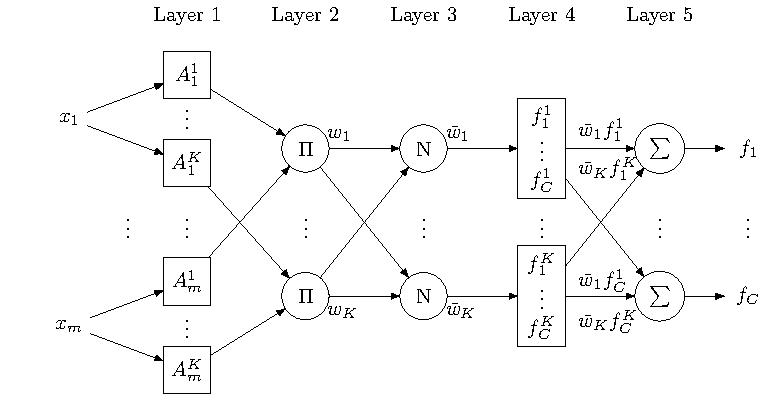
\includegraphics[width=\hsize]{anfis_architecture_classification.pdf}
\caption{\label{fig: ANFIS_architecture}多クラス分類のためのANFIS構造.}
\end{figure}

ANFIS~\cite{Jang1993}は,図\ref{fig: ANFIS_architecture}に示すように,5層のニューラルネットワークアーキテクチャによって多クラス分類のためのTS-FIS推定~\cite{Angelov2004}を実現する.
各ノードの機能は,以下のようにまとめられる.

\vspace{3mm}
\noindent
\textbf{Layer 1:}

各ノード関数は,与えられた入力$x_j$が言語ラベル$A_j^k$を満足する度合いを出力する.
ファジィメンバシップ関数は,最大値が1,最小値が0のベル型関数,またはガウス関数を用いることが一般的である.
この層でのパラメータは,「前提部パラメータ」と呼ばれ,逆伝播における勾配降下法によって更新する.

本論文では,個体$i$の$j$番目の入力$x_{ij}$の$k$番目のルールへのメンバシップ度を表現するため,前提部パラメータ$a_{kj}, b_{kj}, c_{kj}$から成る,以下で与えられるベル型関数を用いる.

\begin{equation}
	\mu_{kj} (x_{ij}) = \frac{1}{1+\left( \left(\frac{x_{ij}-c_{kj}}{a_{kj}} \right)^2 \right)^{b_{kj}}}
\end{equation}

\vspace{3mm}
\noindent
\textbf{Layer 2:}

この層の全ノードは,入力値を乗算し,その積をルール$k$の発火強度$w_{ki} = \prod_{j=1}^m \mu_{kj} (x_{ij})$として出力する.
この層では,更新すべきパラメータはない.

\vspace{3mm}
\noindent
\textbf{Layer 3:}

この層での全ノードは,すべてのルールの発火強度の和が1となるように,ルールの発火強度を正規化する.
それゆえ,個体$i$のルール$k$に対する正規化発火強度$\bar{w}_{ki}$は,発火強度$w_{ki}$を用いて,$\bar{w}_{ki} = w_{ki} / \sum_{\ell=1}^K w_{\ell i}$のように計算される.
この層においても,更新すべきパラメータはない.

\vspace{3mm}
\noindent
\textbf{Layer 4:}

各ノード関数は,各ルールの結果を以下のように出力する.

\begin{equation}
	\bar{w}_{ki} \times f_{c}^k (\bmath{x}_{i}) = \bar{w}_{ki} r_{k}^c, \quad c=1, \dots, C
\end{equation}
この層におけるパラメータ$r_{k}^c$は,「結論部パラメータ」と呼ばれ,順伝播における最小二乗推定によって更新される.

\vspace{3mm}
\noindent
\textbf{Layer 5:}

この層の$C$個のノードは,すべての入力値の総和を出力値として計算する.
つまり,各システムの出力は,以下のように与えられる$K$個のルールすべての出力のファジィメンバシップによる重み付け平均から求められる.

\begin{equation}
	\hat{y}_{ic} = f_c (\bmath{x}_{i}) = \sum_{k=1}^K \bar{w}_{ki} \times f_{c}^k (\bmath{x}_{i}), \; c=1, \dots, C
\end{equation}

また,個体$i$の出力クラス$class_i$は,次のように分類される.

\begin{equation}
	class_i = {\rm argmax}_{c} \; \hat{y}_{ic}
\end{equation}

\subsection{ノイズファジィクラスタリング}

FCM法~\cite{Bezdek81a}は,各クラスタ$k$がそのクラスタ中心$\bmath{b}_k$によって表され,クラスタ基準が入力データ$\bmath{x}_i$とクラスタ中心$\bmath{b}_k$の間のユークリッド距離によって定義される$k$個の分割をファジィに推定するためのクラスタリングアルゴリズムである.最小化すべき目的関数は,以下のように与えられる.
\begin{equation}
\begin{aligned}[b]
J_{fcm} &=\sum_{k=1}^{K} \sum_{i=1}^{n} u_{k i}^{\theta} d_{k i} \\
&=\sum_{k=1}^{K} \sum_{i=1}^{n} u_{k i}^{\theta}\left\|\bmath{x}_{i}-\bmath{b}_{k}\right\|^{2}
\end{aligned}
\label{eq: object FCM}
\end{equation}
$u_{ki}$ ($u_{ki} \in [0, 1]$)は個体$i$のクラスタ$k$へのファジィメンバシップであり,$\sum_{k=1}^K u_{ki} = 1$となるよう制約されている.
$\theta$ ($\theta > 1$)は,分割のファジィ度を調整する重み付け指数であり,$\theta$の値を大きくすると,クラスタの境界がファジィになる一方,$\theta$を1に近づけると,$k$-meansのクリスプな分割~\cite{MacQueen67}に近づく.
一般的に,$\theta = 2$がファジィ度として用いられる~\cite{Bezdek81a}.

クラスタリングアルゴリズムは,ファジィメンバシップ$u_{ki}$とクラスタ中心$\bmath{b}_k$を反復的に更新するような,交互最適化の原理に基づいて構築される.
Noise fuzzy $c$-means (NFCM)~\cite{Dave91,Dave97}は,FCM法の拡張手法であり,ノイズクラスタを追加することにより,ノイズ除去を実現している.
全個体から等しい距離$\gamma$をもつ追加のノイズクラスタのインデックスを$K+1$とする.NFCM法の目的は,以下で与えられる目的関数を最小化することによって,$K+1$個のクラスタを抽出することである.
\begin{equation}
\begin{aligned}[b]
J_{n f c m} &=\sum_{i=1}^{n}\left(\sum_{k=1}^{K} u_{k i}^{\theta} d_{k i}+u_{K+1, i}^{\theta} \gamma\right) \\
&=\sum_{i=1}^{n}\left(\sum_{k=1}^{K} u_{k i}^{\theta} \| \boldsymbol{x}_{i}-\boldsymbol{b}_{k} \|^{2}+u_{K+1, i}^{\theta} \gamma\right)
\end{aligned}
\label{eq: object NFCM}
\end{equation}
$u_{K+1, i}$は,個体$i$のノイズクラスタへのファジィメンバシップであり,メンバシップ値は以下の確率的制約の下で計算される.
\begin{equation}
	\sum_{k=1}^{K+1} u_{ki} = 1
\label{eq: sum-to-one condition for noise FCM}
\end{equation}
個体$i$が,$K$個の正常なクラスタすべてから$\gamma$以上離れている場合,その個体は,ノイズクラスタへ割り当てられ,大きなファジィメンバシップ$u_{K+1, i}$が与えられる.
そのため,$K$個の正常なクラスタのクラスタ中心をノイズの影響なしに計算できる.

ここで,正常なクラスタが1つだけであるとすると,NFCM法は,初期点をランダムにとるロバストな平均ベクトルを推定することを目的としたpossibilistic $c$-means (PCM)~\cite{Krishnapuram93}とみなすことができる.

同様の考え方が,確率的推定を用いないノイズクラスタリングに基づくロバストな分析にも応用された.
ファジィ主成分分析(Fuzzy PCA)によるロバストな$k$-means法~\cite{Honda2010_IEEE-TFS}は,個体$i$の非ノイズ度とノイズ度を表す通常のファジィメンバシップ$u_i$とその補数$1-u_i$をそれぞれ利用するようなロバストなPCAを,$k$-means法に導入しており,その目的関数は,以下の式で与えられる.

\begin{equation}
	J_{rkm} = \sum_{i=1}^n \left( (1-u_i)^\theta \gamma + u_i^\theta \sum_{k=1}^K \sum_{i \in G_k} || \bmath{x}_i - \bmath{b}_k||^2 \right)
\end{equation}

\end{document}

\documentclass{ujarticle}
\usepackage{sotsuron}
\pagestyle{myheadings}
\twocolumn
\begin{document}
\section{ノイズファジィクラスタリングによるロバストなANFIS分類器}

本論文では,ノイズファジィクラスタリングの概念に基づいた多クラス分類のための新しいロバストなANFISモデルを提案する.
分類器設計の目的は,教師クラスラベルを出来る限り正確に予測することであるが,実際の適用において全個体に正しいラベルを割り当てることは,しばしば困難であったりコストがかかる.
若しくは,ノイズを含む信頼のできない教師ラベルをもつこともある.
このようにノイズの多い場合,分類器を教師クラスラベルが信頼できないノイズ個体の影響を無視するように構築する必要がある.
本論文では,ノイズファジィクラスタリングの概念を導入することにより,ANFISによる分類器をノイズラベルに対してロバスト化する新しいアプローチを提案する.

\subsection{目的関数}

各個体の非ノイズ度を推定するため,提案法では,ノイズクラスタリング基準としてANFISの目的関数を利用し,以下に示すようなハイブリッドな目的関数を用いる.
%
\begin{equation}
	J_{ranfis} = \sum_{i=1}^n \left( (1-u_i)^\theta \gamma + u_i^\theta \sum_{c=1}^C (y_{ic} - \hat{y}_{ic})^2 \right)
\end{equation}
%
$u_i$は,個体$i$の非ノイズ度を表し,$u_i \in [0, 1]$の条件をもつ.
$u_i=1$と$u_i=0$は,それぞれ完全に非ノイズ個体・ノイズ個体であることを示している.
$\theta$は,FCM法と同様,ファジィ度であり,$\theta > 1$の値をとる.
また,$\theta$の値が大きいほど,ファジィなメンバシップ値となる.
$\gamma$は,ノイズ感度の重みであり,$\gamma$の値が小さいほど,多数の信頼できない個体が除去される.
すなわち,基準$\sum_{c=1}^C (y_{ic} - \hat{y}_{ic})^2$が,$\gamma$より大きければ,個体$i$はANFISのモデル推定から除去される.

\subsection{前提部パラメータの更新}

Layer 1の前提部パラメータ$\phi_{kj} \in \{ a_{kj}, b_{kj}, c_{kj} \}$は,各入力$(\bmath{x}_i, \bmath{y}_i)$に対して以下のような逆誤差伝播学習における勾配降下法に基づいて更新される.
%
\begin{equation}
	\phi_{kj} \leftarrow \phi_{kj} - \tau \frac{\partial d_i}{\partial \phi_{kj}}
\label{eq: premise parameters learning}
\end{equation}
%
$\tau$は学習率であり,$d_i$は,次のように求められる個体ごとのコストである.
%
\begin{equation}
	d_i = \sum_{c=1}^C (y_{ic} - \hat{y}_{ic})^2
\end{equation}
%
連鎖律の下で,$\frac{\partial d_i}{\partial \phi_{kj}}$は,次のように分解される.
%
\begin{equation}
\begin{aligned}[b]
\frac{\partial d_{i}}{\partial \phi_{k j}} &=\sum_{t=1}^{K} \frac{\partial d_{i}}{\partial \bar{w}_{t i}} \frac{\partial \bar{w}_{t i}}{\partial w_{k i}} \frac{\partial w_{k i}}{\partial \mu_{k j}\left(x_{i j}\right)} \frac{\partial \mu_{k j}\left(x_{i j}\right)}{\partial \phi_{k j}} \\
&=\frac{\partial w_{k i}}{\partial \mu_{k j}\left(x_{i j}\right)} \frac{\partial \mu_{k j}\left(x_{i j}\right)}{\partial \phi_{k j}} \sum_{t=1}^{K} \frac{\partial d_{i}}{\partial \bar{w}_{t i}} \frac{\partial \bar{w}_{t i}}{\partial w_{k i}}
\end{aligned}
\end{equation}
%
ここで,新しく導入されたパラメータ$u_i$は,$\frac{\partial d_i}{\partial \bar{w}_{ti}}$についてしか関係がない.
%
\begin{equation}
\begin{aligned}[b]
\frac{\partial d_{i}}{\partial \bar{w}_{t i}} &=\frac{\partial}{\partial \bar{w}_{t i}}\left(u_{i}^{\theta} \sum_{c=1}^{C}\left(y_{i c}-\hat{y}_{i c}\right)^{2}\right) \\
&=\frac{\partial}{\partial \bar{w}_{k i}}\left(u_{i}^{\theta} \sum_{c=1}^{C}\left(y_{i c}-\sum_{s=1}^{K} \bar{w}_{s i} r_{s}^{c}\right)^{2}\right) \\
&=-2 u_{i}^{\theta} \sum_{c=1}^{C}\left(y_{i c}-\sum_{s=1}^{K} \bar{w}_{s i} r_{s}^{c}\right)
\end{aligned}
\end{equation}
%
他の要素は,従来のANFISと同じ方法で計算される.

\subsection{結論部パラメータの更新}

Layer 4では,結論部パラメータ$\bmath{r}_c = (r_{1}^c, \dots, r_{K}^c)^\top$が,最小二乗推定に基づいて更新され,目的関数は,以下のように変形される.
%
\begin{equation}
\begin{aligned}[b]
J_{ranfis} &=\sum_{i=1}^{n}\left(\left(1-u_{i}\right)^{\theta} \gamma+u_{i}^{\theta} \sum_{c=1}^{C}\left(y_{i c}-\hat{y}_{i c}\right)^{2}\right) \\
&=\sum_{c=1}^{C} \sum_{i=1}^{n} u_{i}^{\theta}\left(y_{i c}-\sum_{k=1}^{K} \bar{w}_{k i} r_{k}^{c}\right)^{2} \\
& \hspace{30mm} +\sum_{i=1}^{n}\left(1-u_{i}\right)^{\theta} \gamma \\
&=\sum_{c=1}^{C}\left(\tilde{\bmath{y}}_{c}-W \bmath{r}_{c}\right)^{\top} U\left(\tilde{\boldsymbol{y}}_{c}-W \bmath{r}_{c}\right) \\
& \hspace{30mm} +\sum_{i=1}^{n}\left(1-u_{i}\right)^{\theta} \gamma
\end{aligned}
\end{equation}
%
$\tilde{\bmath{y}}_c$は,$n$次元ベクトル$\tilde{\bmath{y}}_c=(y_{1c}, \dots, y_{nc})^\top$である.
$W$は,$n \times K$行列$W=\{ \bar{w}_{ik} \}$であり,$U$は,$i$番目の対角要素が$u_i^\theta$の$n \times n$対角行列である.
$\bmath{r}_c$は,以下のように更新される.
%
\begin{equation}
  \bmath{r}_c = (W^\top U W)^{-1} W^\top U \tilde{\bmath{y}}_c
\label{eq: LSE of coefficient vector}
\end{equation}
%

\subsection{ファジィメンバシップ更新}

非ノイズメンバシップ度$u_i$は,単一クラスタのノイズクラスタリングの概念に基づいて次のように更新される.
%
\begin{equation}
  u_{i} = \left( 1 + \left( \frac{d_i}{\gamma} \right)^{\frac{1}{\theta-1}} \right)^{-1}
\label{eq: non-noise membership calculation}
\end{equation}
%

\subsection{アルゴリズム}

上記の更新則に従い,提案法の手順を以下のサンプルアルゴリズムにまとめた.

\vspace{5mm}
\noindent
\textbf{[A Robust ANFIS Classifier Based on Noise Fuzzy Clustering]}

\begin{description}
	\item[Step 1.] ファジィ度$\theta$,ノイズ感度$\gamma$,ルール数$K$,学習率$\tau$,終了基準$\varepsilon$を設定する.
	\item[Step 2.] FCM法を実行し,初期前提部パラメータを推定する.
	\item[Step 3.] 提案法のロバスト化ANFIS分類器のパラメータを,更新則が収束するまで実行することにより推定する.
	\begin{description}
		\item[Step 3-1.] 非ノイズメンバシップ$u_{i}$をすべて$u_{i}=1$, $i=1, \dots, n$と初期化する.
		\item[Step 3-2.] 結論部パラメータ$\bmath{r}_c$を(\ref{eq: LSE of coefficient vector})式により更新する.
		\item[Step 3-3.] (\ref{eq: premise parameters learning})式の勾配降下法により,前提部パラメータ$\phi_{kj} \in \{ a_{kj}, b_{kj}, c_{kj} \}$を更新する.
		\item[Step 3-4.] 非ノイズ度$u_{i}$, $i=1, \dots, n$を(\ref{eq: non-noise membership calculation})式により更新する.
		\item[Step 3-5.] $ J_{ranfis}^{OLD} - J_{ranfis}^{NEW} < 0$であれば終了する
    .そうでなければ,\textbf{Step 3-2}に戻る.
	\end{description}

\end{description}

\end{document}

\documentclass{ujarticle}
\usepackage{sotsuron}
\pagestyle{myheadings}
\twocolumn
\begin{document}
\section{数値実験}
\subsection{実験方法}

UCI Machine Learning Repository~\cite{UCI_repository2019}から入手可能なIrisデータを用いて数値実験を行った.Iris-setosa,Iris-versicolor,Iris-virginicaの3種類のクラス($C=3$)それぞれ50サンプルずつから構成され,計150個体から構成されている.
また,各個体は,4次元の特徴量($m=4$)で表現されている.
ANFISによる分類器の分類性能を調べるため,Irisデータセットを3つのクラスからそれぞれ40個体をランダムに選択した120個体($n=120$)からなる訓練データと,残りの30個体からなるテストデータに分割した.
ANFISによる分類器を訓練データによって構築し,その汎化性能をテストデータによって評価した.

提案法におけるノイズロバスト性は,以下のように調べた.
訓練データの一部のクラスラベルをランダムに変更し,そのノイズの多い訓練データを用いてANFISによる分類器を構築した.
本実験では,10\%(12ノイズ個体),20\%(24ノイズ個体),30\%(36ノイズ個体),40\%(48ノイズ個体),50\%(60ノイズ個体)の5種類のノイズ比率を用いた.
また,テストデータには元のラベルをそのまま利用しており,ノイズを含んでいない.

ANFIS分類器は,3種類のクラスをもっているため,ルール数$K=3$として分類器の出力:
\[f_c^k, \quad c=1,2,3, \quad k=1,2,3,\]
となるよう構築した.
クラス数$C$は,ルール数$K$と対応することが理想的である.
ファジィ度と学習率は,それぞれ$\theta = 2$,$\tau = 0.00001$と設定した.

\subsection{分類性能の比較}

ノイズを含まない元の訓練データとノイズを含む訓練データに対して,従来法のANFIS分類器と提案法のANFIS分類器を構築した.
その分類性能を,訓練データでは表\ref{tab: classification ratios for training},テストデータでは表\ref{tab: classification ratios for test}に示した.

\begin{table*}[!htbp]
\caption{訓練データに対する分類性能の比較}
\label{tab: classification ratios for training}
\centering
{\tabcolsep = 2.5mm
\begin{tabular}{c||c|c|c|c|c|c}\hline%\cline{3-11}
ノイズ比率	& original& 10\% & 20\%	& 30\% 	& 40\% & 50\%    \\\hline\hline
従来法	& 96.7\% & 86.7\% & 76.7\% & 70.8\% & 58.3\% & 48.3\%    \\\hline
提案法 & 97.5\% & 86.7\% & 76.7\% & 67.5\% & 59.2\% & 51.7\%	 \\\hline
\end{tabular}
}
\end{table*}

表\ref{tab: classification ratios for training}から従来法と提案法のANFISモデルは,どちらも訓練データにノイズラベルを含まない場合,高い分類性能を達成している.
また,データセットにノイズラベルを含む場合,
\[(分類性能)\approx 100\%-(ノイズ比率)\]
によって分類性能を考えることができる.そのため,ノイズを含んでいたとしても非ノイズ個体に対しては,どちらのモデルにおいてもほぼ完璧な分類性能を達成している.

\begin{table*}[!htbp]
\caption{テストデータに対する分類性能の比較}
\label{tab: classification ratios for test}
\centering
{\tabcolsep = 2.5mm
\begin{tabular}{c||c|c|c|c|c|c}\hline%\cline{3-11}
ノイズ比率	& original& 10\% & 20\%	& 30\% 	& 40\% & 50\%    \\\hline\hline
従来法 & 100.0\% & 96.7\% & 96.7\% & 90.0\% & 86.7\% & 76.7\%    \\\hline
提案法 & 100.0\% & 100.0\% & 96.7\% & 93.3\% & 90.0\% & 86.7\%	 \\\hline
\end{tabular}
}
\end{table*}

一方テストデータに対しては,表\ref{tab: classification ratios for test}に示したように,そのデータにノイズを含まないにも関わらず,従来法と提案法のANFISによる分類器の汎化性能が低下している.
これは,訓練データのノイズラベルに分類器が過適合し,非ノイズ個体の分類に失敗することがあるためである.

提案法では,テストデータに対する汎化性能を従来法より向上させることに成功した.
すなわち,従来法においては,誤ったラベルをもつノイズ個体の影響によって汎化性能が低下したが,提案法においては,ノイズ個体を適切に識別し分類器の構築においてその影響を除去できている.

\subsection{メンバシップ関数の比較}

ここでは,従来法と提案法によるANFISから得られたファジィメンバシップ関数を比較する.
図\ref{fig: membership of conventional ANFIS}と図\ref{fig: membership of proposed robust ANFIS}では,4つの変量$(x_1, \dots, x_4)$についてのルールごとのメンバシップ関数$\mu_{kj} (x_{j})$を,ノイズなしの元の訓練データと50\%のノイズラベルを含む訓練データで比較している.

いずれの手法においても,ノイズのないデータでは,なめらかなメンバシップ関数を構築することができたが,従来法のモデルでは,データセットにノイズを含むとき属性$x_1$のルール2において,尖った形状の関数が得られた.
このような尖った形状は,何らかのノイズ個体に対して過適合を起こしうる.
対して提案法では,訓練データにノイズラベルが含まれている場合でも変わらず,なめらかなメンバシップ関数を構築している.
このノイズに強い特徴は,ANFISによる分類器のノイズが多いデータセットへの汎化性能の向上に役立つと考えられる.

\begin{figure*}[!htb]
  \begin{minipage}{0.45\hsize}
    \centering
    \includegraphics[width=\textwidth]{Final_mf_anfis_00.png}
    \subcaption{original (ノイズなし)}
  \end{minipage}
  \begin{minipage}{0.45\hsize}
    \centering
    \includegraphics[width=\textwidth]{Final_mf_anfis_50.png}
    \subcaption{ノイズ 50$\%$}
  \end{minipage}
  \caption{従来法ANFISのファジィメンバシップ関数.}
  \label{fig: membership of conventional ANFIS}
\end{figure*}

\begin{figure*}[!htb]
  \begin{minipage}{0.45\hsize}
    \centering
    \includegraphics[width=\textwidth]{Final_mf_noise_00.png}
    \subcaption{original (ノイズなし)}
  \end{minipage}
  \begin{minipage}{0.45\hsize}
    \centering
    \includegraphics[width=\textwidth]{Final_mf_noise_50.png}
    \subcaption{ノイズ 50$\%$}
  \end{minipage}
  \caption{提案法ANFISのファジィメンバシップ関数.}
  \label{fig: membership of proposed robust ANFIS}
\end{figure*}

\end{document}

\documentclass{ujarticle}
\usepackage{sotsuron}
\pagestyle{myheadings}
\twocolumn
\begin{document}
\section{まとめ}

本論文では,ノイズファジィクラスタリングの概念を導入することで,ANFISによる分類器をノイズのあるクラスラベルに対するロバスト化を目的として改良した.
各個体の非ノイズ度をFCM法のようにメンバシップ値で表し,これをANFISのモデル推定に利用してノイズの影響を除去する.
提案法の特徴を,数値実験において従来法と比較すると,テストデータの分類性能が向上することが示された.
また,ANFISの前提部のメンバシップ関数を比較すると,従来のモデルではノイズ個体に過適合し,尖った形状となった一方,提案法では,ノイズの多い訓練データに対してもなめらかな関数を維持することができた.

今後の課題としては,クラス比が不均衡であったり,クラスの重複があるような他種類のデータに対するノイズ感度を調査することが挙げられる.

\section*{謝辞}

本研究は本学工学域電気電子系学類情報工学課程の本多克宏教授,生方誠希准教授の御指導のもとに行われたものであり,心より感謝の意を表します.

\end{document}



\begin{thebibliography}{99}
\bibitem{Jang1993}
Jang, J.-S. R.: ANFIS: Adaptive-network-based fuzzy inference system. IEEE Transactions on Systems, Man and Cybernetics, \textbf{23}(3), 665--685 (1993)

\bibitem{Takagi1985}
Takagi, T., Sugeno, M.: Fuzzy identification of systems and its applications to modeling and control. IEEE Transactions on Systems, Man and Cybernetics, \textbf{15}, 116--132 (1985)

\bibitem{Angelov2004}
Angelov, P., Xydeas, C., Filev, D.: On-line identification of MIMO evolving Takagi-Sugeno fuzzy models. In: 2004 IEEE International Conference on Fuzzy Systems, \textbf{1}, 55--60, (2004)

\bibitem{Honda_ICIEV2021}
Honda, K., Hyakutake, S., Ubukata, S., Notsu, A.: A hybrid robust ANFIS based on noise fuzzy clustering, In: 10th International Conference on Informatics, Electronics \& Vision and 5th International Conference on Imaging, Vision \& Pattern Recognition, \textbf{81}, 1--7 (2021)

\bibitem{Bezdek81a}
Bezdek, J. C.: Pattern Recognition with Fuzzy Objective Function Algorithms, Plenum Press (1981)

\bibitem{Miyamoto_book08}
Miyamoto, S., Ichihashi, H., Honda, K.: Algorithms for Fuzzy Clustering, Springer (2008)

\bibitem{Dave91}
Dav\'e, R. N.: Characterization and detection of noise in clustering. Pattern Recognition Letters, \textbf{12}(11), 657--664 (1991)

\bibitem{Dave97}
Dav\'e, R. N., Krishnapuram, R.: Robust clustering methods: a unified view. IEEE Trans. on Fuzzy Systems, \textbf{5}, 270--293 (1997)

\bibitem{Holland77}
Holland, P. W., Welsch, R. E.: Robust regression using iteratively reweighted least-squares. Communications in Statistics, \textbf{A6}(9), 813--827 (1977)

\bibitem{Honda2010_IEEE-TFS}
Honda, K., Notsu, A., Ichihashi, H.: Fuzzy PCA-guided robust $k$-means clustering. IEEE Trans. Fuzzy Systems, \textbf{18}(1), 67--79 (2010)

\bibitem{Angelov2008}
Angelov, P. P., Zhou, X.: Evolving fuzzy-rule-based classifiers from data streams. IEEE Transactions on Fuzzy Systems, \textbf{16}(6), 1462--1475 (2008)

\bibitem{MacQueen67}
MacQueen, J. B.: Some methods of classification and analysis of multivariate observations. Proc. of 5th Berkeley Symposium on Math. Stat. and Prob., 281--297 (1967)

\bibitem{Krishnapuram93}
Krishnapuram, R., Keller, J. M.: A possibilistic approach to clustering. IEEE Trans. on Fuzzy Systems,  \textbf{1}, 98--110 (1993)

\bibitem{UCI_repository2019}
Dua, D., Graff, C.: UCI Machine Learning Repository. Irvine, CA: University of California, School of Information and Computer Science (2019)  \url{http://archive.ics.uci.edu/ml} Last accessed 30 Nov 2021

\end{thebibliography}
\end{document}
